\chapter{RECIPROCAL LATTICE}

\section{Reciprocal Lattice}
Physical propertiess of crystalline solids are different in different directions in them. i.e., crystalline solids are anisotropic with respect to many of the physical properies. Hence a method of representation od planes and directions has become inevitable in the studies of crystal structure.
One can indicate the orientation of a of parallel planes by their common normal and the interplanar spacing by restricting the length of the normals proportionately.\\
If the normals are drawn, to each set of parallel planes, from a common origin and their lengths. are made proportional to reciprocal of the respectitve interplanar spacings, the points at the ends of these normals form a lattice array. Since the distances in this array are reciprocal to distances in the crystal, the array is called the 'reciprocal lattice' of the crystal.\\
The points in the reciprocal lattice are called reciprocal lattice points. These points in three dimensional space form the reciprocal lattice space. This reciprocal lattice space is also called the $k$-space. From the concept of reciprocal lattice it may be understood that the 'coordinates of points' in the reciprocal lattice space are defined by $(h k l)$, the Miller indices.\\
\subsubsection{Geometrical Construction}
With what we have discussed until now, the general rules for constructing the reciprocal lattice may be formulated by the following steps:
\begin{enumerate}
	\item Fix up some point in the direct lattice as a common origin.
	\item From this common origin draw normals to each and every set of parallel planes in the direct lattice.
	\item Fix the length of each normal equal to the reciprocal of the interplanar spacing $\left(1 / d_{hk l)}\right)$ of the set of parallel planes $(h k l)$ it represents.
	\item Put a point at the end of each normal.
\end{enumerate}
The collection of all these points in space is the reciprocal lattice space. The concept of reciprocal lattice is useful for redefining the Bragg's condition and introducing the concept of Brillouin Zone.

\subsection{Reciprocal lattice to $\mathrm{SC}$ lattice}

The primitive translation vectors $f$ a simple cubic lattice may be written as

The reciprocal lattice vectors the $\mathrm{SC}$ lattice are obtained\\
$\left.\begin{array}{lll}
	\vec{a}=a \hat{i} & \vec{b}=b \hat{j} \quad \vec{c}=a \hat{k} ; & \left.V=|\vec{a} \cdot \vec{b} \times \vec{c}|=a^{3} \quad \begin{array}{l}
		\hat{i} \cdot \hat{i}=\hat{j} \cdot \hat{j}=\hat{k} \cdot \hat{k}=1 \\
		\hat{i} \cdot \hat{j}=\hat{j} \cdot \hat{k}=\hat{k} \cdot \hat{i}=0
	\end{array}\right\}
\end{array}\right\}$
\begin{align}
a^{*}&=2 \pi \frac{\vec{b} \times \vec{c}}{|a \cdot b \times c|}=2 \pi \frac{a \hat{j} \times a \hat{k}}{a^{3}}=\frac{2 \pi}{a} \hat{i} \label{reciprocal lattice-1}\\
b^{*}&=2 \pi \frac{\vec{c} \times \vec{a}}{|\vec{a} \cdot \vec{b} \times \vec{c}}=\frac{2 \pi}{a} \hat{J}\label{reciprocal lattice-2} \\
c^{*}&=2 \pi \frac{\vec{a} \times \vec{b}}{\mid \vec{a} \cdot(\vec{b} \times \vec{c} \mid}=\frac{2 \pi}{a} \vec{K} \label{reciprocal lattice-3}
\end{align}
Equation \ref{reciprocal lattice-1}, \ref{reciprocal lattice-2} \& \ref{reciprocal lattice-3} indicate that all the three reciprocal lattice vectors are equal in magnitude which means that the reciprocal lattice to SC lattice is also simple cubic but with lattice constant equal to $2 \pi /$ a.

\subsection{Reciprocal lattice to $\mathrm{BCC}$ lattice}

The primitive translation vectors of a body centred cubic lattice


\begin{align*}
a^{\prime}&=a / 2(\hat{i}+\hat{j}-\hat{k}) \\
b^{\prime}&=a / 2(-\hat{i}+\hat{j}+\hat{k}) \\
c^{\prime}&=a / 2(\hat{i}-\hat{j}+\hat{k}) \\
\text { use } \vec{b} \times \vec{c}&=\left[\begin{array}{lll}\hat{i} & \hat{j} & \hat{k} \\b_{x} & b_{y} & b_{z} \\c_{x} & c_{y} & c_{z}\end{array}\right]\\
V&=(\vec{a} \cdot \vec{b} \times \vec{c})=a / 2(\hat{i}+\hat{j}-\hat{k}) \cdot\left[\frac{a^{2}}{4}(-\hat{i}+\hat{j}+\hat{k}) \times(\hat{i}-\hat{j}+\hat{k})\right] \\
&=\left.\hat{i}\left[b_{y}\left(c_{z}-c_{z} b_{z}\right)\right]-\hat{j}\left[b_{x} c_{z}-c_{x} b_{z}\right)\right]+\hat{k}\left[b_{x} c_{y}-c_{x} b_{y}\right]\\
\text{Reciprocal lattice vector} &=\frac{\mathrm{a}^{3}}{2}\\
a^{*}&=2 \pi \frac{b^{\prime} \times c^{\prime}}{(\vec{a} \cdot \vec{b} \times \vec{c})}=\frac{2 \pi\left(a^{2} / 2\right)}{a^{3} / 2}(\hat{l}+\hat{j})\\&=\frac{2 \pi}{a}(\hat{l}+\hat{j})\\
b^{*}&=2 \pi \frac{c^{\prime} \times a^{\prime}}{(\vec{a} \cdot \vec{b} \times \vec{c})}=\frac{2 \pi}{a}(\hat{j}+\hat{k})\\
c^{*} &=2 \pi \frac{a^{\prime} \times b^{\prime}}{\left(a\cdot b^{\prime} \times \vec{c}\right)}=\frac{2 \pi}{a}(\hat{k}+\hat{l})\\
\end{align*}
Thus reciprocal lattice to a bcc lattice is fcc lattice

\subsection{Reciprocal lattice to $\mathrm{FCC}$ lattice:}

The primitive translations vectors of an fcc lattice are
\begin{align*}
a^{\prime}&=a / 2(\hat{l}+\hat{j}), \quad b^{\prime}=a / 2(\hat{j}+\hat{k}), \quad  c^{\prime}=a / 2(\hat{k}+\hat{l})  \\
V&=|\vec{a} \cdot \vec{b} \times \vec{c}|=\frac{a^{3}}{4}\\
a^{*}&=2 \pi \frac{b^{\prime} \times \vec{c}}{\left(a^{\prime} \cdot b^{\prime} \times \vec{c}\right)}=2 \pi \frac{\left(a^{2} / 4\right)(\hat{l}+\hat{j}-\hat{k})}{a^{3} / 4}=\frac{2 \pi}{a}(\hat{l}+\hat{j}-\hat{k}) \\
b^{\prime}&=2 \pi \frac{c^{\prime} \times a^{\prime}}{a^{\prime} \cdot b^{\prime} \times c^{\prime}}=\frac{2 \pi}{a}(-\hat{l}+\hat{j}+\hat{k})\\
c^{\prime}&=2 \pi \frac{a^{\prime} \times b^{\prime}}{a \cdot\left(b^{\prime} \times \vec{c}\right)}=\frac{2 \pi}{a}(\hat{l}-\hat{j}+\hat{k})
\end{align*}
Thus reciprocal lattice to an fcc lattice is a bcc lattice.

\section{Properties of Reciprocal lattice}
\begin{enumerate}
	\item Each point in a reciprocal lattice corresponding to particular set of parallel planes of the direct lattice.
	\item The distance of a reciprocal lattice point from an arbitrarily fixed origin is inversely proportional to the interplanar spacing of the corresponding parallel planes of the direct lattice.
	\item The volume of a unit cell of the reciprocal lattice is inversely proportional to the corresponding unit cell of the direct lattice.
	\item The unit cell of the reciprocal lattice need not be a parallelepiped. It is customary to deal with Winger-Feitz cell of reciprocal lattice which constitutes the Brillouin zone.
\end{enumerate}
\begin{example}
	 Two-dimensional lattice has the basis vectors $a=2 \hat{x} \quad b=\hat{x}+2 \hat{y}$. Find the reciprocal lattice vector.\\
	 $\pi=\left(\hat{x}-\frac{\hat{y}}{2}\right), \pi \hat{y}$
\end{example}

\section{Bragg's Law in Reciprocal Lattice}
The Bragg's diffraction condition obtained earlier by considering reflection from parallel lattice plane can be used to express geometrical relationship between the vectors in the reciprocal lattice such a using a Ewald construction.\\
The Bragg's law itself takes a diffraction from in the reciprocal lattice to obtain the modified form of the Bragg's law, we redraw the vector $\overrightarrow{\mathrm{AO}}, \overrightarrow{O \mathrm{~B}}, \overrightarrow{\mathrm{AB}}$ such that each is magnified by a constant factor of $2 \pi$. \\
Let the new vector be $\overrightarrow{\mathrm{AO}}, \overrightarrow{O \mathrm{~B}}$ and $\overrightarrow{\mathrm{AB}}$ respectively as shown in figure, since $\quad \mathrm{AO}=\frac{2 \pi}{\lambda}$, we can represent the wave vector $\mathrm{K}$ by the vector $\overrightarrow{\mathrm{AO}}$. The vector $\overrightarrow{O \mathrm{~B}}$ is the reciprocal vector and is written as $\mathrm{G}$. Thus, according to vector algebra $\overrightarrow{\mathrm{AB}}$ must be equal to $(\mathrm{K}+\mathrm{G})$. For diffraction to occur, the point B' must be on the sphere. i.e.
\begin{figure}[H]
	\centering
	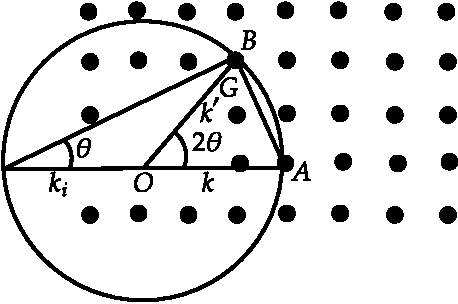
\includegraphics[height=4cm,width=5.5cm]{Brillouin zone 1}
	\caption{Bragg's Law in Reciprocal Lattice}
	\label{Bragg's Law in Reciprocal Lattice}
\end{figure}

\begin{align*}
|\overrightarrow{\mathrm{AB}}|&=|\overrightarrow{\mathrm{AO}}| \\
(K+G)^{2}&=K^{2} \\
K^{2}+2 K \cdot G+G^{2}&=K^{2} \\
2 K \cdot G+G^{2}&=0
\end{align*}
This is the vector form of Bragg's law and is used in construction of the Brillouin zones.
The vector $\overrightarrow{\mathrm{A}^{\prime} \mathrm{B}^{\prime}}$ represents the direction of reflected or scattered beam denting it by $\mathrm{K}^{\prime}$,
\begin{align*}
\text{ We get }K^{\prime}&=K+G\\
\text{Which gives } K^{2}&=K^{2}\\ 
\text{Or } K^{\prime}-K&=n a\\
\text{And }K^{\prime}-K&=K=G
\end{align*}
This indicates that the scattering does not change the magnitude of wave vector $\mathrm{K}$, only its direction is changed, the scattered wave differs from the incident by a reciprocal lattice vector $G$. 
\subsection{Brillouin Zones}
A Brillouin Zone is the locus of all those $\mathrm{K}$-values in the reciprocal lattice which are Bragg's reflected.\\
"The $1^{\text {st }}$ Brillouin Zone is the smallest volume entired by planes that are the perpendicular bisector of the reciprocal lattice vectors drawn from the origin".
\subsection{Brillouin zones for $\mathrm{SC}$ :}
\begin{align*}
a&=a \hat{i}, b=a \hat{j}, c=a \hat{k}\\
a^{*}&=\left(\frac{2 \pi}{a}\right) i, \quad b^{*}=\left(\frac{2 \pi}{a}\right) j, c^{*}=\left(\frac{2 \pi}{a}\right) \hat{k}
\intertext{Therefore, the reciprocal lattice vector is written as}
\mathrm{G}&=\left(\frac{2 \pi}{a}\right)(h \hat{i}+k \hat{j}+l \hat{k})\\
\intertext{Where $\mathrm{h}, \mathrm{k}$ and $l$ are integers. The wave vector $\mathrm{k}$ can be expressed as}
K&=K_{x} \hat{i}+K_{y} \hat{j}+K_{z} \hat{k}
\intertext{From the Bragg's condition we have} 
2 \mathrm{~K} \cdot \mathrm{G}+\mathrm{G}^{2}&=0\\
\frac{4 \pi}{a}\left[\left(K_{x} \hat{i}+K_{y} \hat{j}+K_{z} \hat{k}\right) \cdot(h \hat{i}+k \hat{j}+l \hat{k})\right]&+\frac{4 \pi}{a^{2}}\left(h^{2}+k^{2}+l^{2}\right)=0\\
h K_{x}+k K_{y}+l K_{z}&=-\left(\frac{\pi}{a}\right)\left(h^{2}+k^{2}+l^{2}\right)
\intertext{The $\mathrm{K}$-values which are Bragg reflected are obtained by considering all possible combination of $\mathrm{h}$ and $\mathrm{K}$.}
\intertext{For $\mathrm{h}=\pm 1$ and $\mathrm{k}=l=0, K_{x}=\pm \pi / \mathrm{a}$ and $K_{y} \& K_{z}$ is arbitrary.}
\intertext{For $\mathrm{h}=l=0$ and $\mathrm{k}=\pm 1, K_{y}=\pm \pi / \mathrm{a}$ and $K_{x} \& K_{z}$ is arbitrary}
\intertext{For $\mathrm{h}=\mathrm{k}=0$ and $\mathrm{l}=\pm 1, K_{z}=\pm \pi / \mathrm{a}$ and $K_{x} \& K_{y}$ is arbitrary}
\end{align*}
These six planes construct a cube of length $2 \pi / \mathrm{a}$, thus the $1^{\text {st }}$ B.Z. of the simple cubic is also a simple cubic with volume $(2 \pi / a)^{3}$. 

\subsection{Brillouin Zone of $\mathrm{BCC}$ lattice:}
\begin{align*}
a&=\frac{a}{2}(\hat{i}+\hat{j}-\hat{k}) \quad a^{*}=\left(\frac{2 \pi}{a}\right)(\hat{i}+\hat{j})\\
b&=\frac{a}{2}(-\hat{i}+\hat{j}+\hat{k}) \quad b^{*}=\left(\frac{2 \pi}{a}\right)(\hat{j}+\hat{k})\\
c^{*}&=\left(\frac{2 \pi}{a}\right)(\hat{k}+\hat{i}) \quad  c=\frac{a}{2}(\hat{i}-\hat{j}+\hat{k})
\intertext{The G-type vector is}
\mathrm{G}&=\mathrm{ha}^{*}+\mathrm{kb}^{*}+\mathrm{lc}^{*}\\
&= \left(\frac{2 \pi}{a}\right)[(h+k) \hat{i}+(k+l) \hat{j}+(h+l) \hat{k}]
\end{align*}
Shortest non-zero $\mathrm{G}^{\mathrm{s}}$ are the following eight vector,
$$\frac{2 \pi}{a}(\pm \hat{i} \pm \hat{j}) \quad ;\quad \frac{2 \pi}{a}(\pm \hat{j} \pm \hat{k}) \quad;\quad \frac{2 \pi}{a}(\pm \hat{k} \pm \hat{i})$$
The first B.Z. is the region enclosed by the normal bisector planes to these 12 vectors. This zone has the sphere of a regular 12 faced solid and is called Rhombic dodecahedron.

\subsection{ Brillouin Zone of $\mathbf{F C C}$ lattice:}
\begin{align*}
a&=\frac{a}{2}(\hat{i}+\hat{j}) \quad a^{*}\\&=\left(\frac{2 \pi}{a}\right)(\hat{i}+\hat{j}-\hat{k})\\
b&=\frac{a}{2}(\hat{j}+\hat{k}) \quad b^{*}\\&=\left(\frac{2 \pi}{a}\right)(-\hat{i}+\hat{j}+\hat{k})\\
c&=\frac{a}{2}(\hat{k}+\hat{i}) \quad c^{*}\\&=\left(\frac{2 \pi}{a}\right)(\hat{i}-\hat{j}+\hat{k})
\intertext{The G-type vector is,}
\mathrm{G}&=\mathrm{ha}^{*}+\mathrm{kb}^{*}+\mathrm{lc}^{*}\\&=
\left(\frac{2 \pi}{a}\right)[(h-k+l) \hat{i}+(h+k-l) \hat{j}+(-h+k+l) \hat{k}]
\end{align*}
Shortest non-zero $\mathrm{G}^{\mathrm{ss}}$ are the following eight vector
$$
\frac{2 \pi}{a}(\hat{i} \pm \hat{j} \pm \hat{k})
$$
The boundaries of the $1^{\text {st }}$ B.Z. are determined mostly by the normal bisector planes to the above 8 vectors.\\
However, the corners of the octahedral obtained in this manner are truncated by the planes which are normal bisectors to the following 6 reciprocal lattice vectors.
$$
\left(\frac{2 \pi}{a}\right)(\pm 2 \hat{i}) ;\left(\frac{2 \pi}{a}\right)(\pm 2 \hat{j}) ;\left(\frac{2 \pi}{a}\right)(\pm 2 \hat{k})
$$
The $1^{\text {st }}$ B.Z. has the shape of Truncated Octahedron 
\begin{exercise}
	The lattice vector of graphene can be written as
	$$
	\vec{a}=\frac{3 a}{2}\left(\hat{x}+\frac{1}{\sqrt{3}} \hat{y}\right): \vec{b}=\frac{3 a}{2}\left(\hat{x}-\frac{1}{\sqrt{3}} \hat{y}\right)
	$$
	Where the carbon-carbon distance is $a=1 \cdot 42 \AA$. Find the area of the Brillouin zone is
\end{exercise}
\begin{answer}
	\begin{align*}
	\text{Given, } \vec{a}&=\frac{3 a}{2}\left(\hat{x}+\frac{1}{\sqrt{3}} \hat{y}\right) \\ \vec{b}&=\frac{3 a}{2}\left(\hat{x}-\frac{1}{\sqrt{3}} \hat{y}\right)\\
	\text{Assume, }\vec{c}&=\hat{k}
	\intertext{The reciprocal lattice vectors are}
	\overrightarrow{a^{*}}&=2 \pi \frac{\vec{b} \times \vec{c}}{\vec{a} \cdot(\vec{b} \times \vec{c})}\\&=\frac{2 \pi}{3 a}(\hat{x}+\sqrt{3} \hat{y}) \text { and } \overrightarrow{b^{*}}=2 \pi \frac{\vec{c} \times \vec{a}}{\vec{a} \cdot(\vec{b} \times \vec{c})}\\&=\frac{2 \pi}{3 a}(\hat{x}+\sqrt{3} \hat{y})
	\intertext{The area of the Brillouin zone is}
	A&=\overrightarrow{a^{*} \times b^{*}}=\left(\frac{2 \pi}{3 a}\right)^{2}[(\hat{x}-\sqrt{3} \hat{y}) \times(\hat{x}-\sqrt{3} \hat{y})] \\
	&=\left(\frac{2 \pi}{3 a}\right)^{2}[0-\sqrt{3} \hat{z}-\sqrt{3} \hat{z}]=\left(\frac{2 \pi}{3 a}\right)^{2}[-2 \sqrt{3} \hat{z}] \\
	\text { Area, }|A|&=\left(\frac{2 \pi}{3 a}\right)^{2}(2 \sqrt{3})\\&=\frac{8 \pi^{2}}{3 \sqrt{3} a^{2}}\\&=7 \cdot 54(\hat{A})^{-2}
	\end{align*}
\end{answer}

\begin{exercise}
A hypothetical two-dimensional lattice has basis vector $\vec{a}_{1}=a \hat{x}$ and $\vec{a}_{2}=\frac{a}{2}(\hat{x}+\sqrt{3} \hat{y})$. Find the area of it's reciprocal lattice
\end{exercise}
\begin{answer}
	\begin{align*}
	\vec{a}_{1}&=a \hat{x}\\
	\vec{a}_{2}&=\frac{a}{2}(\hat{x}+\sqrt{3} \hat{y})\\
	\text{Assume,} \vec{a}_{3}&=\hat{z}\\
	\text{Now, } \vec{a}_{1} \cdot\left(\vec{a}_{2} \times \vec{a}_{3}\right)&=a \hat{x} \cdot\left[\frac{a}{2}(\hat{x}+\sqrt{3} \hat{y}) \times \hat{z}\right]\\&=\frac{a^{2}}{2} \hat{x} \cdot[-\hat{y}+\sqrt{3} \hat{x}]=\frac{a^{2}}{2}[0+\sqrt{3}]\\&=\frac{\sqrt{3} a^{2}}{2}\\
	\vec{a}_{1}^{*}&=2 \pi \frac{\vec{a}_{2} \times \vec{a}_{3}}{\vec{a}_{1} \cdot\left(\vec{a}_{2} \times \vec{a}_{3}\right)}\\&=2 \pi \frac{(\sqrt{3} \hat{x}-\hat{y}) \frac{a}{2}}{\frac{\sqrt{3}}{2} a^{2}}\\&=\frac{2 \pi}{a}\left(\hat{x}-\frac{\hat{y}}{\sqrt{3}}\right) \\
	\text{and } \vec{a}_{2}^{*}\\&=2 \pi \frac{\vec{a}_{3} \times \vec{a}_{1}}{\vec{a}_{1} \cdot\left(\vec{a}_{2} \times \vec{a}_{3}\right)}\\&=\frac{4 \pi}{\sqrt{3} a} \hat{y}
	\intertext{Area of reciprocal cell is}
	A^{*}&=\vec{a}_{1}^{*} \times \vec{a}_{2}^{*}\\&=\frac{2 \pi}{a}\left(\hat{x}-\frac{\hat{y}}{\sqrt{3}}\right) \times \frac{4 \pi}{\sqrt{3} a} \hat{y}\\&=\frac{8 \pi^{2}}{\sqrt{3} a^{2}}(\hat{z})
	\end{align*}
\end{answer}
\begin{exercise}
	The two-dimensional lattice of Graphene is arranged in a Honeycomb lattice where carbon occupy the vertices as shown below. The positive vectors are $\vec{a}$ and $\vec{a}_{2}$. The lattice spacing is $a$. Find the area of the Brilliouin zone
\end{exercise}
\begin{answer}
	 The primitive vectors are written as
	

	\begin{align*}
	&\vec{a}_{1}=\sqrt{3} a \cos 30^{\circ} \hat{i}+\sqrt{3} a \cos 60^{\circ} \hat{j}=\frac{\sqrt{3}}{2} a(\sqrt{3} \hat{i}+\hat{j}) \\
	&\vec{a}_{2}=\sqrt{3} a \cos 30^{\circ} \hat{i}-\sqrt{3} a \cos 60^{\circ} \hat{j}=\frac{\sqrt{3}}{2} a(\sqrt{3} \hat{i}-\hat{j})
	\intertext{Area of the primitive cell is}
	A&=\left|\vec{a}_{1} \times \vec{a}_{2}\right|\\&=\frac{3 \sqrt{3}}{2} a^{2}
	\intertext{The reciprocal lattice vectors are (assume $\vec{a}_{3}=\hat{k}$ )}
	\vec{a}_{1}^{*}&=\frac{2 \pi}{a} \frac{\vec{a}_{2} \times \vec{a}_{3}}{V}=\frac{2 \pi}{3 a}(\hat{i}+\sqrt{3} \hat{j}) \\
	\vec{a}_{2}^{*}&=\frac{2 \pi}{a} \frac{\vec{a}_{3} \times \vec{a}_{1}}{V}=\frac{2 \pi}{3 a}(\hat{i}-\sqrt{3} \hat{j})
	\intertext{area of the Brilliouin zone is}
	A^{*}&=\left|\vec{a}_{1}^{*} \times \vec{a}_{2}^{*}\right|\\&=\frac{4 \pi^{2}}{9 a^{2}}|(\hat{i}+\sqrt{3} \hat{j}) \times(\hat{i}-\sqrt{3} \hat{j})|\\&=\frac{4 \pi^{2}}{9 a^{2}} \cdot 2 \sqrt{3}\\&=\frac{8 \pi^{2}}{3 \sqrt{3} a^{2}}
	\end{align*}
\end{answer}








